% Author: Dominik Harmim <harmim6@gmail.com>


\documentclass[%
    10pt, xcolor=pdflatex, hyperref={unicode}, aspectratio=169%
]{beamer}


\usepackage{newcent}
\usepackage[utf8]{inputenc}
\usepackage[british]{babel}
\usepackage[T1]{fontenc}
\usepackage{xcolor}
\usepackage{listings}

\definecolor{bluekeywords}{rgb}{.13, .13, 1}
\definecolor{greencomments}{rgb}{0, .5, 0}
\definecolor{redstrings}{rgb}{.9, 0, 0}
\lstset{
    basicstyle=\ttfamily,
    keywordstyle=\color{bluekeywords},
    commentstyle=\color{greencomments},
    stringstyle=\color{redstrings},
    backgroundcolor=\color{white},
    language=C++,
    tabsize=2,
    escapeinside={<@}{@>},
    frame=trBL,
    columns=fullflexible,
    showstringspaces=true,
    keepspaces=true,
    showspaces=false,
    showtabs=false,
    breaklines=true,
    breakatwhitespace=true
}


%%%%%%%%%%%%%%%%%%%%%%%%%%%%%%%%%%%%%%%%%%%%%%%%%%%%%%%%%%%%%%%%%%%%%%%%%%%%%%%%
\usetheme{FIT}

\title[%
    Advanced Static Analysis of Atomicity in Concurrent Programs through
    Facebook Infer%
]{%
    Advanced Static Analysis of Atomicity in Concurrent Programs through
    Facebook Infer%
}
\subtitle{\texorpdfstring{SEP\,---\,Term Project}{SEP - Term Project}}

\author{\texorpdfstring{%
    Dominik Harmim \\
    \footnotesize{Supervisor: prof. Ing. Tomáš Vojnar, Ph.D.}%
}{Dominik Harmim; Supervisor: prof. Ing. Tomáš Vojnar, Ph.D.}}

\institute{%
    xharmi00@stud.fit.vutbr.cz \\
    Brno University of Technology, Faculty of Information Technology%
}

\date{\today}
%%%%%%%%%%%%%%%%%%%%%%%%%%%%%%%%%%%%%%%%%%%%%%%%%%%%%%%%%%%%%%%%%%%%%%%%%%%%%%%%


\begin{document}


%%%%%%%%%%%%%%%%%%%%%%%%%%%%%%%%%%%%%%%%%%%%%%%%%%%%%%%%%%%%%%%%%%%%%%%%%%%%%%%%
\section{Title Page}
\frame[plain]{\titlepage}


%%%%%%%%%%%%%%%%%%%%%%%%%%%%%%%%%%%%%%%%%%%%%%%%%%%%%%%%%%%%%%%%%%%%%%%%%%%%%%%%
\section{Motivation}
\begin{frame}[fragile]{Motivation}
    \begin{itemize}
        \item
            Detecting and checking desired \alert{atomicity of call
            sequences}.

            \smallskip

            \begin{itemize}\setlength\itemsep{1em}
                \item
                    Often required in \emph{concurrent programs}.

                \item
                    Violation may cause \emph{nasty errors}.
            \end{itemize}
    \end{itemize}

    \medskip

    \begin{columns}
        \begin{column}{.6 \linewidth}
            \centering

            \begin{lstlisting}
void invoke(char *method) {
    <@\texttt{\ldots}@>
    if (server.<@\textbf{is\_registered}@>(method)) {
        server.<@\textbf{invoke}@>(method);
    }
    <@\texttt{\ldots}@>
}
            \end{lstlisting}
        \end{column}

        \begin{column}{.4 \linewidth}
            \centering

            The sequence of \texttt{\textbf{is\_registered}} and
            \texttt{\textbf{invoke}} should be \alert{executed
            atomically}.

            \medskip

            {\footnotesize
                If \emph{not locked}, the method can be
                unregistered by a~\emph{concurrent thread}.
            }
        \end{column}
    \end{columns}
\end{frame}


%%%%%%%%%%%%%%%%%%%%%%%%%%%%%%%%%%%%%%%%%%%%%%%%%%%%%%%%%%%%%%%%%%%%%%%%%%%%%%%%
\section{Facebook Infer}
\begin{frame}{Facebook Infer}
    \begin{columns}
        \begin{column}{1 \linewidth}
            \begin{itemize}
                \item
                    An open-source \alert{static analysis framework}
                    for \emph{interprocedural analyses}.

                    \smallskip

                    \begin{itemize}\setlength\itemsep{1em}
                        \item
                            Based on \alert{abstract interpretation}.
                    \end{itemize}
            \end{itemize}
        \end{column}

        \hfill
    \end{columns}

    \begin{columns}
        \begin{column}{.55 \linewidth}
            \begin{itemize}\setlength\itemsep{2em}
                \item
                    \alert{Highly scalable}.

                    \smallskip

                    \begin{itemize}\setlength\itemsep{1em}
                        \item
                            Follows principles of \emph{compositionality}.

                        \item
                            Computes function \emph{summaries} bottom-up
                            on call trees.
                    \end{itemize}

                \item
                    Supports Java, C, C++, and Objective-C.
            \end{itemize}
        \end{column}

        \begin{column}{.45 \linewidth}
            \begin{center}
                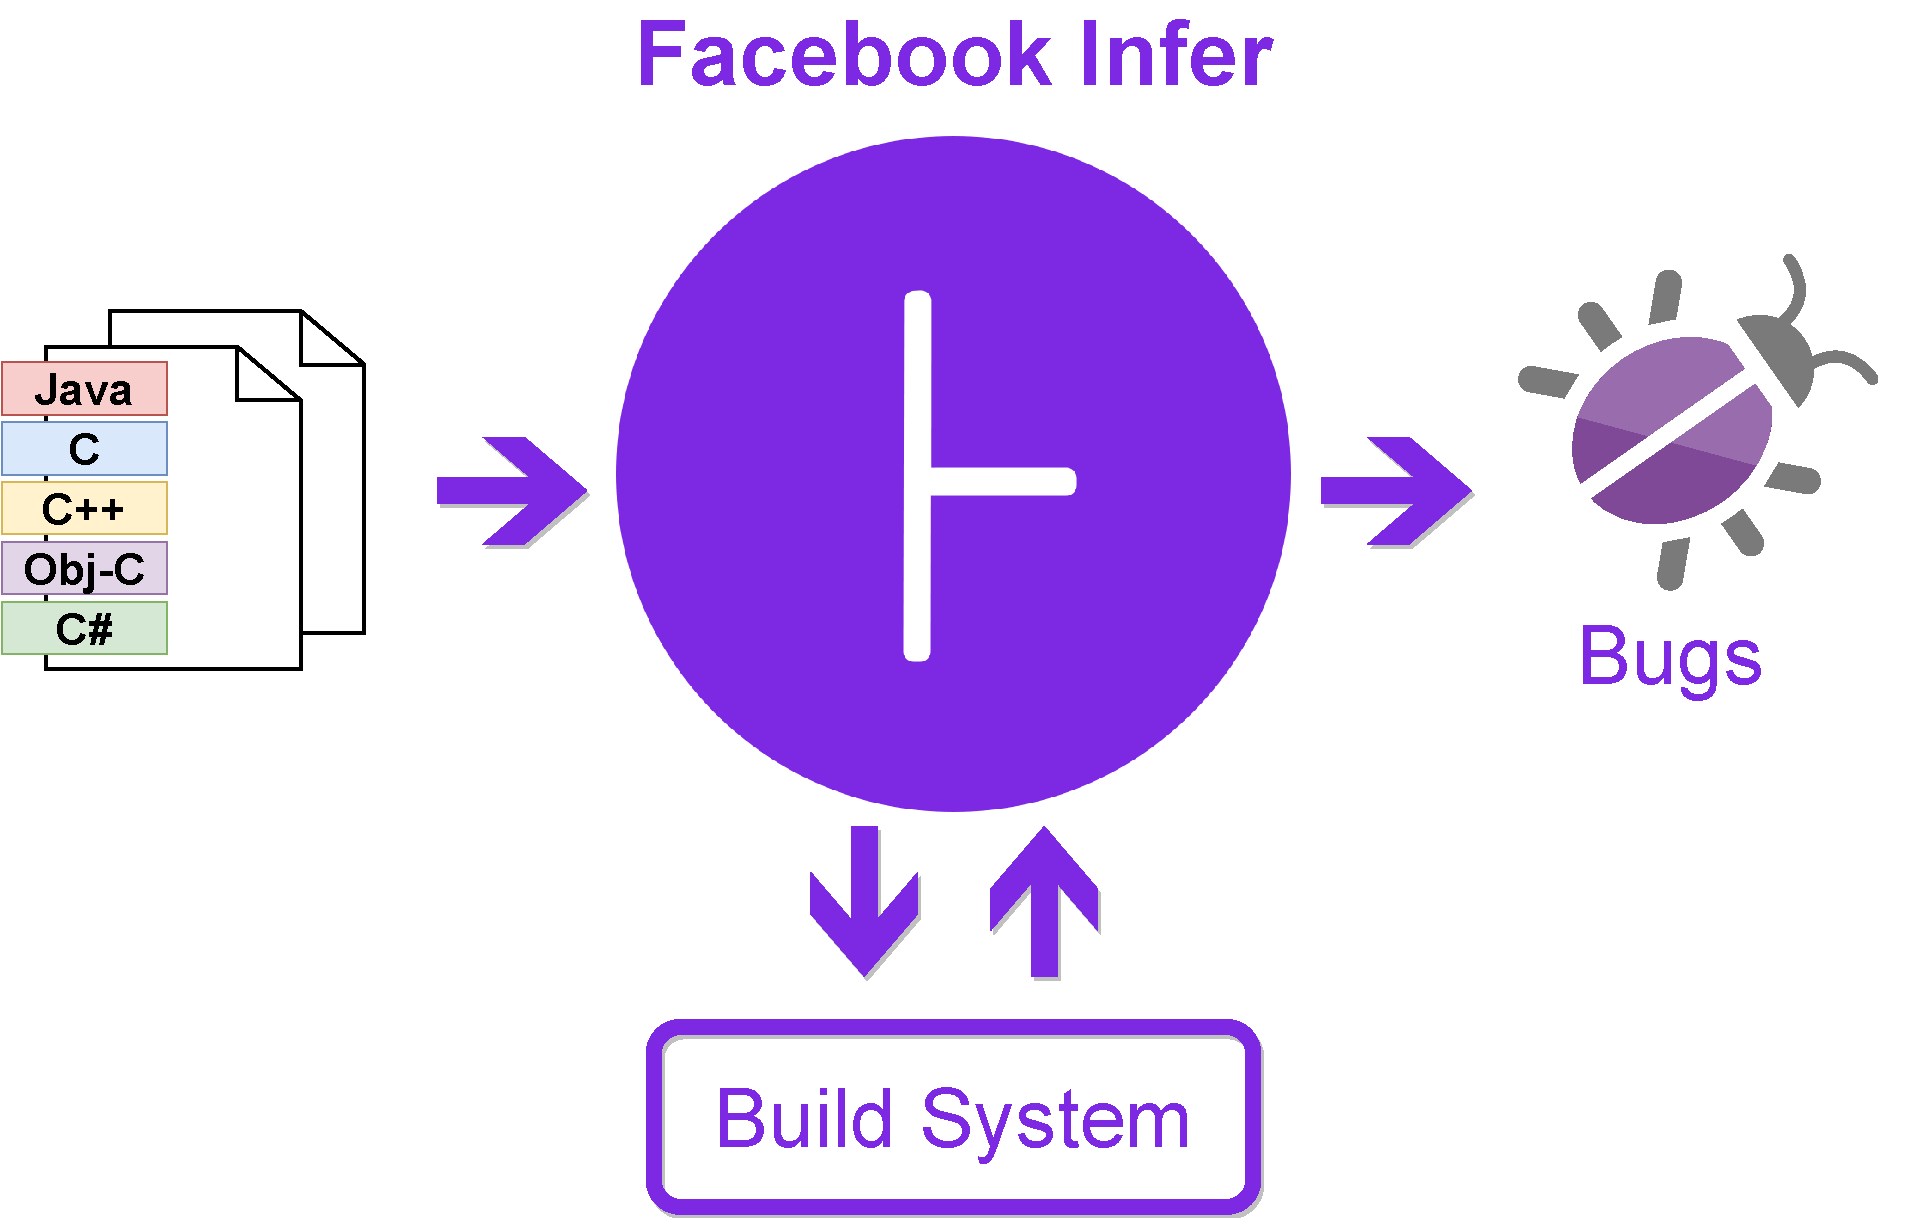
\includegraphics[width=1 \linewidth]{img/infer.pdf}
            \end{center}
        \end{column}
    \end{columns}
\end{frame}


%%%%%%%%%%%%%%%%%%%%%%%%%%%%%%%%%%%%%%%%%%%%%%%%%%%%%%%%%%%%%%%%%%%%%%%%%%%%%%%%
\section{Atomer: Atomicity Violations Analyser}
\begin{frame}{Atomer: Atomicity Violations Analyser}
    \begin{itemize}\setlength\itemsep{3em}
        \item
            A~\emph{Facebook Infer plugin} created within
            a~bachelor's thesis.

        \item
            \textbf{Assumption}: \alert{Call sequences} executed
            \emph{atomically once} should be executed
            \emph{always atomically}.

        \item
            Implemented for \emph{C/C++/Java} programs
            that use classical \emph{mutual exclusion mechanisms}.
    \end{itemize}
\end{frame}


%%%%%%%%%%%%%%%%%%%%%%%%%%%%%%%%%%%%%%%%%%%%%%%%%%%%%%%%%%%%%%%%%%%%%%%%%%%%%%%%
\section{Atomer: Two Phases of the Analysis}
\begin{frame}[fragile]{Atomer: Two Phases of the Analysis}
    \begin{columns}
        \begin{column}[T]{.5 \linewidth}
            \centering

            \begin{enumerate}
                \item
                    Detection of \alert{atomic call sets}.
            \end{enumerate}

            \begin{itemize}
                \item
                    Approximates \emph{sequences} by \emph{sets}.

                \item
                    \textbf{Summaries}: (\textcolor{brown}{set of all
                    calls}, \textcolor{magenta}{set of atomic call sets})
            \end{itemize}

            \begin{lstlisting}
void f() {
    <@\texttt{\textcolor{red}{\textbf{lock}}}@>(L);
    f1(); f1(); f2();
    <@\texttt{\textcolor{red}{\textbf{unlock}}}@>(L);
    a();
    <@\texttt{\textcolor{red}{\textbf{lock}}}@>(L);
    b(); c();
    <@\texttt{\textcolor{red}{\textbf{unlock}}}@>(L);
}
            \end{lstlisting}

            \textbf{\texttt{\footnotesize
                \alert{summary\textsubscript{f}}: \\
                (\textcolor{brown}{\{f1, f2, a, b, c\}},
                \textcolor{magenta}{\{\{f1, f2\}, \{b, c\}\}})
            }}
        \end{column}

        \begin{column}[T]{.5 \linewidth}
            \centering

            \begin{enumerate}\setcounter{enumi}{1}
                \item
                    Detection of \alert{atomicity violations}.
            \end{enumerate}

            \begin{itemize}
                \item
                    Looks for \emph{non-atomic pairs of calls}
                    assumed to run atomically.

                \item
                    \textbf{Summaries}: (\textcolor{orange}{set of
                    first calls}, \textcolor{violet}{set of last
                    calls}, \textcolor{red}{set of atomicity
                    violations})
            \end{itemize}

            \begin{lstlisting}
void g() {
    a();
    <@\texttt{\textcolor{red}{\textbf{f1}}}@>(); <@\texttt{\textcolor{red}{\textbf{f2}}}@>();
    b();
}
            \end{lstlisting}

            \textbf{\texttt{\footnotesize
                \alert{summary\textsubscript{g}}: \\
                (\textcolor{orange}{\{a\}},
                \textcolor{violet}{\{b\}},
                \textcolor{red}{\{(f1, f2)\}})
            }}
        \end{column}
    \end{columns}
\end{frame}


%%%%%%%%%%%%%%%%%%%%%%%%%%%%%%%%%%%%%%%%%%%%%%%%%%%%%%%%%%%%%%%%%%%%%%%%%%%%%%%%
\section{Atomer: New Main Features}
\begin{frame}{Atomer: New Main Features}
    \begin{itemize}\setlength\itemsep{3em}
        \item
            \alert{Approximation} \emph{atomic calls sequences} by
            \emph{sets}.

        \item
            Support for \alert{C++ and Java locks} (earlier supported
            only \emph{Pthreads}).

            \smallskip

            \begin{itemize}\setlength\itemsep{1em}
                \item
                    \textbf{C++}: \texttt{std::mutex, std::lock,
                    std::lock\_guard, std::shared\_mutex,
                    std::timed\_mutex, std::recursive\_mutex,
                    std::unique\_lock, \ldots}

                \item
                    \textbf{Java}: monitors (\texttt{synchronized}),
                    \texttt{java.util.concurrent.locks.Lock,
                    java.util.concurrent.locks.ReentrantLock, \ldots}
            \end{itemize}

        \item
            Distinguishes \alert{multiple (nested) locks} using
            \emph{syntactic access paths}.
    \end{itemize}
\end{frame}


%%%%%%%%%%%%%%%%%%%%%%%%%%%%%%%%%%%%%%%%%%%%%%%%%%%%%%%%%%%%%%%%%%%%%%%%%%%%%%%%
\section{Experimental Evaluation}
\begin{frame}{Experimental Evaluation}
    \textbf{Earlier Evaluation:}
    \medskip
    \begin{itemize}\setlength\itemsep{1em}
        \item
            The \alert{correctness} was first verified on
            \emph{hand-crafted} programs.

        \item
            \alert{Real-life low-level concurrent~C} programs from
            a~Debian-based benchmark suite.

            \smallskip

            \begin{itemize}\setlength\itemsep{1em}
                \item
                    Several \emph{potential atomicity violations} have
                    been found.
            \end{itemize}
    \end{itemize}

    \bigskip

    \textbf{New Evaluation:}
    \medskip
    \begin{itemize}\setlength\itemsep{1em}
        \item
            More had-crafted programs to verify the correctness of
            the new features.

        \item
            \alert{Real-life Java} programs\,--\,\alert{Apache Cassandra}
            and \alert{Tomcat} ($ \sim $200k LOC).

            \smallskip

            \begin{itemize}\setlength\itemsep{1em}
                \item
                    Successfully rediscovered \emph{already fixed
                    reported real bugs}.

                \item
                    So far quite some \alert{false alarms}\,--\,need
                    to increase accuracy.
            \end{itemize}
    \end{itemize}
\end{frame}


%%%%%%%%%%%%%%%%%%%%%%%%%%%%%%%%%%%%%%%%%%%%%%%%%%%%%%%%%%%%%%%%%%%%%%%%%%%%%%%%
\section{Future Goals}
\begin{frame}{Future Goals}
    \begin{itemize}\setlength\itemsep{3em}
        \item
            Further analysis of \alert{real-life programs} with
            an effort to find and report \alert{new bugs}.

            \smallskip

            \begin{itemize}\setlength\itemsep{1em}
                \item
                    GNU Coreutils/Binutils, Mozilla, MariaDB, \ldots

                \item
                    Focus on \emph{library containers concurrency
                    restrictions} related to method calls.
            \end{itemize}

        \item
            Increase \alert{accuracy}.

            \smallskip

            \begin{itemize}\setlength\itemsep{1em}
                \item
                    Distinguishing the \emph{context of called
                    functions} by considering \emph{formal parameters}
                    (using \emph{syntactic access paths}).

                \item
                    \alert{Ranking} of atomic functions.
            \end{itemize}
    \end{itemize}
\end{frame}


\end{document}
